% $Header: /cvsroot/latex-beamer/latex-beamer/examples/beamerexample5.tex,v 1.22 2004/10/08 14:02:33 tantau Exp $

\documentclass[11pt]{beamer}

\usetheme{Darmstadt}

\usepackage{times}
\usefonttheme{structurebold}

%\usepackage[english]{babel}
\usepackage[portuges]{babel}
\usepackage{pgf,pgfarrows,pgfnodes,pgfautomata,pgfheaps}
\usepackage{amsmath,amssymb}
%\usepackage[latin8]{inputenc}
\usepackage[utf8]{inputenc}
\usepackage{graphicx}

\setbeamercovered{dynamic}

\newcommand{\Lang}[1]{\operatorname{\text{\textsc{#1}}}}

\newcommand{\Class}[1]{\operatorname{\mathchoice
  {\text{\sf \small #1}}
  {\text{\sf \small #1}}
  {\text{\sf #1}}
  {\text{\sf #1}}}}

\newcommand{\NumSAT}      {\text{\small\#SAT}}
\newcommand{\NumA}        {\#_{\!A}}

\newcommand{\barA}        {\,\bar{\!A}}

\newcommand{\Nat}{\mathbb{N}}
\newcommand{\Set}[1]{\{#1\}}

\pgfdeclaremask{tu}{beamer-tu-logo-mask}
\pgfdeclaremask{computer}{beamer-computer-mask}
\pgfdeclareimage[interpolate=true,mask=computer,height=2cm]{computerimage}{beamer-computer}
\pgfdeclareimage[interpolate=true,mask=computer,height=2cm]{computerworkingimage}{beamer-computerred}
\pgfdeclareimage[mask=tu,height=.5cm]{logo}{logounesp}

\logo{\pgfuseimage{logo}}

\title{Métodos de Operadores}
\author{Ney Lemke}
\institute[IBB-UNESP]{%
    Mec\^anica Qu\^antica}
\date{2013}                                

\colorlet{redshaded}{red!25!bg}
\colorlet{shaded}{black!25!bg}
\colorlet{shadedshaded}{black!10!bg}
\colorlet{blackshaded}{black!40!bg}

\colorlet{darkred}{red!80!black}
\colorlet{darkblue}{blue!80!black}
\colorlet{darkgreen}{green!80!black}

\def\radius{0.96cm}
\def\innerradius{0.85cm}

\def\softness{0.4}
\definecolor{softred}{rgb}{1,\softness,\softness}
\definecolor{softgreen}{rgb}{\softness,1,\softness}
\definecolor{softblue}{rgb}{\softness,\softness,1}

\definecolor{softrg}{rgb}{1,1,\softness}
\definecolor{softrb}{rgb}{1,\softness,1}
\definecolor{softgb}{rgb}{\softness,1,1}

\newcommand{\Bandshaded}[2]{
  \color{shadedshaded}
  \pgfmoveto{\pgfxy(-0.5,0)}
  \pgflineto{\pgfxy(-0.6,0.1)}
  \pgflineto{\pgfxy(-0.4,0.2)}
  \pgflineto{\pgfxy(-0.6,0.3)}
  \pgflineto{\pgfxy(-0.4,0.4)}
  \pgflineto{\pgfxy(-0.5,0.5)}
  \pgflineto{\pgfxy(4,0.5)}
  \pgflineto{\pgfxy(4.1,0.4)}
  \pgflineto{\pgfxy(3.9,0.3)}
  \pgflineto{\pgfxy(4.1,0.2)}
  \pgflineto{\pgfxy(3.9,0.1)}
  \pgflineto{\pgfxy(4,0)}
  \pgfclosepath
  \pgffill

  \color{black}  
  \pgfputat{\pgfxy(0,0.7)}{\pgfbox[left,base]{#1}}
  \pgfputat{\pgfxy(0,-0.1)}{\pgfbox[left,top]{#2}}
}

\newcommand{\Band}[2]{
  \color{shaded}
  \pgfmoveto{\pgfxy(-0.5,0)}
  \pgflineto{\pgfxy(-0.6,0.1)}
  \pgflineto{\pgfxy(-0.4,0.2)}
  \pgflineto{\pgfxy(-0.6,0.3)}
  \pgflineto{\pgfxy(-0.4,0.4)}
  \pgflineto{\pgfxy(-0.5,0.5)}
  \pgflineto{\pgfxy(4,0.5)}
  \pgflineto{\pgfxy(4.1,0.4)}
  \pgflineto{\pgfxy(3.9,0.3)}
  \pgflineto{\pgfxy(4.1,0.2)}
  \pgflineto{\pgfxy(3.9,0.1)}
  \pgflineto{\pgfxy(4,0)}
  \pgfclosepath
  \pgffill

  \color{black}  
  \pgfputat{\pgfxy(0,0.7)}{\pgfbox[left,base]{#1}}
  \pgfputat{\pgfxy(0,-0.1)}{\pgfbox[left,top]{#2}}
}

\newcommand{\BaenderNormal}
{%
  \pgfsetlinewidth{0.4pt}
  \color{black}
  \pgfputat{\pgfxy(0,5)}{\Band{input tapes}{}}
  \pgfputat{\pgfxy(0.35,4.6)}{\pgfbox[center,base]{$\vdots$}}
  \pgfputat{\pgfxy(0,4)}{\Band{}{}}

  \pgfxyline(0,5)(0,5.5)
  \pgfxyline(1.2,5)(1.2,5.5)
  \pgfputat{\pgfxy(0.25,5.25)}{\pgfbox[left,center]{$w_1$}}

  \pgfxyline(0,4)(0,4.5)
  \pgfxyline(1.8,4)(1.8,4.5)        
  \pgfputat{\pgfxy(0.25,4.25)}{\pgfbox[left,center]{$w_n$}}
  \ignorespaces}

\newcommand{\BaenderZweiNormal}
{%
  \pgfsetlinewidth{0.4pt}
  \color{black}
  \pgfputat{\pgfxy(0,5)}{\Band{Zwei Eingabeb\~AƒÂƒ\~A‚¤nder}{}}
  \pgfputat{\pgfxy(0,4.25)}{\Band{}{}}

  \pgfxyline(0,5)(0,5.5)
  \pgfxyline(1.2,5)(1.2,5.5)
  \pgfputat{\pgfxy(0.25,5.25)}{\pgfbox[left,center]{$u$}}

  \pgfxyline(0,4.25)(0,4.75)
  \pgfxyline(1.8,4.25)(1.8,4.75)        
  \pgfputat{\pgfxy(0.25,4.5)}{\pgfbox[left,center]{$v$}}
  \ignorespaces}

\newcommand{\BaenderHell}
{%
  \pgfsetlinewidth{0.4pt}
  \color{black}
  \pgfputat{\pgfxy(0,5)}{\Bandshaded{input tapes}{}}
  \color{shaded}
  \pgfputat{\pgfxy(0.35,4.6)}{\pgfbox[center,base]{$\vdots$}}
  \pgfputat{\pgfxy(0,4)}{\Bandshaded{}{}}

  \color{blackshaded}
  \pgfxyline(0,5)(0,5.5)
  \pgfxyline(1.2,5)(1.2,5.5)
  \pgfputat{\pgfxy(0.25,5.25)}{\pgfbox[left,center]{$w_1$}}

  \pgfxyline(0,4)(0,4.5)
  \pgfxyline(1.8,4)(1.8,4.5)        
  \pgfputat{\pgfxy(0.25,4.25)}{\pgfbox[left,center]{$w_n$}}
  \ignorespaces}

\newcommand{\BaenderZweiHell}
{%
  \pgfsetlinewidth{0.4pt}
  \color{black}
  \pgfputat{\pgfxy(0,5)}{\Bandshaded{Zwei Eingabeb\~AƒÂƒ\~A‚¤nder}{}}%
  \color{blackshaded}
  \pgfputat{\pgfxy(0,4.25)}{\Bandshaded{}{}}
  \pgfputat{\pgfxy(0.25,4.5)}{\pgfbox[left,center]{$v$}}
  \pgfputat{\pgfxy(0.25,5.25)}{\pgfbox[left,center]{$u$}}%

  \pgfxyline(0,5)(0,5.5)
  \pgfxyline(1.2,5)(1.2,5.5)

  \pgfxyline(0,4.25)(0,4.75)
  \pgfxyline(1.8,4.25)(1.8,4.75)        
  \ignorespaces}

\newcommand{\Slot}[1]{%
  \begin{pgftranslate}{\pgfpoint{#1}{0pt}}%
    \pgfsetlinewidth{0.6pt}%
    \color{structure}%
    \pgfmoveto{\pgfxy(-0.1,5.5)}%
    \pgfbezier{\pgfxy(-0.1,5.55)}{\pgfxy(-0.05,5.6)}{\pgfxy(0,5.6)}%
    \pgfbezier{\pgfxy(0.05,5.6)}{\pgfxy(0.1,5.55)}{\pgfxy(0.1,5.5)}%
    \pgflineto{\pgfxy(0.1,4.0)}%
    \pgfbezier{\pgfxy(0.1,3.95)}{\pgfxy(0.05,3.9)}{\pgfxy(0,3.9)}%
    \pgfbezier{\pgfxy(-0.05,3.9)}{\pgfxy(-0.1,3.95)}{\pgfxy(-0.1,4.0)}%
    \pgfclosepath%
    \pgfstroke%
  \end{pgftranslate}\ignorespaces}

\newcommand{\SlotZwei}[1]{%
  \begin{pgftranslate}{\pgfpoint{#1}{0pt}}%
    \pgfsetlinewidth{0.6pt}%
    \color{structure}%
    \pgfmoveto{\pgfxy(-0.1,5.5)}%
    \pgfbezier{\pgfxy(-0.1,5.55)}{\pgfxy(-0.05,5.6)}{\pgfxy(0,5.6)}%
    \pgfbezier{\pgfxy(0.05,5.6)}{\pgfxy(0.1,5.55)}{\pgfxy(0.1,5.5)}%
    \pgflineto{\pgfxy(0.1,4.25)}%
    \pgfbezier{\pgfxy(0.1,4.25)}{\pgfxy(0.05,4.15)}{\pgfxy(0,4.15)}%
    \pgfbezier{\pgfxy(-0.05,4.15)}{\pgfxy(-0.1,4.2)}{\pgfxy(-0.1,4.25)}%
    \pgfclosepath%
    \pgfstroke%
  \end{pgftranslate}\ignorespaces}

\newcommand{\ClipSlot}[1]{%
  \pgfrect[clip]{\pgfrelative{\pgfxy(-0.1,0)}{\pgfpoint{#1}{4cm}}}{\pgfxy(0.2,1.5)}\ignorespaces}

\newcommand{\ClipSlotZwei}[1]{%
  \pgfrect[clip]{\pgfrelative{\pgfxy(-0.1,0)}{\pgfpoint{#1}{4.25cm}}}{\pgfxy(0.2,1.25)}\ignorespaces}


\AtBeginSection[]{\frame{\frametitle{Outline}\tableofcontents[current]}}

\begin{document}
\frame{\titlepage}

\frame{\frametitle{Visão Geral} As informações sobre um determinado
  sistema físico podem estar contidas:
  \begin{itemize}
  \item na função de onda $\psi(x)$
  \item na função de onda no espaço de momento $\phi(p)$
  \item nos coeficientes da expansão em termos de autofunções de
    enegia $c_a$
  \end{itemize}
}

\frame{\frametitle{Visão Geral} Usando a notação de Dirac podemos
  representar de forma abstracta essas informações usando o vetor de
  estado:

$$|\psi \rangle$$

ou pelo seu vetor conjugado:

$$\langle \psi |$$

eles são chamados de ``bras'' : $\langle \psi |$ e de ``kets'' $|\psi \rangle$.

Observe que em Inglês ``$\langle$'' e ``$\rangle$'' são chamados de brackets.  }


\frame{\frametitle{Alice no País das maravilhas}
  \begin{tabular}{c c}
    \begin{minipage}{0.45\textwidth}
      \begin{center}
        \begin{description}
        \item[Alice] Would you tell me, please, which way I ought to
          go from here?
        \item[The Cat] That depends a good deal on where you want to
          get to.
        \item[Alice] I don't much care where.
        \end{description}
      \end{center}
    \end{minipage}&
    \begin{minipage}{0.45\textwidth}
      \begin{center}
        \includegraphics[scale=0.6]{alice}
      \end{center}
    \end{minipage}
  \end{tabular}

}

\frame{\frametitle{Alice no País das maravilhas}
  \begin{tabular}{c c}
    \begin{minipage}{0.45\textwidth}
      \begin{center}
        \begin{description}
        \item[The Cat] Then it doesn't much matter which way you go.
        \item[Alice] …so long as I get somewhere.
        \item[The Cat] Oh, you're sure to do that, if only you walk
          long enough.
        \end{description}
      \end{center}
    \end{minipage}&
    \begin{minipage}{0.45\textwidth}
      \begin{center}
        \includegraphics[scale=0.6]{alice}
      \end{center}
    \end{minipage}
  \end{tabular}
}

\frame{\frametitle{Wittgenstein}
  \begin{tabular}{c c}
    \begin{minipage}{0.45\textwidth}
      My propositions are elucidatory in this way: he who understands
      me finally recognizes them as senseless, when he has climbed out
      through them, on them, over them.
\end{minipage}
    \begin{minipage}{0.45\textwidth}
      \begin{center}
        \includegraphics[scale=0.3]{wittgenstein.jpg}
      \end{center}
    \end{minipage}
  \end{tabular}
}

 \frame{\frametitle{Poder da Notação} A notação de Dirac é uma das
  maravilhas modernas, muito mais concisa e intuitiva ela é o melhor
  veículo para transmitir MQ. Mas vamos precisar de um dicionário para
  migrar da nossa notação para a nova notação }

\frame{\frametitle{Dicionário}
  \begin{tabular}{c c}
    \begin{minipage}{0.45\textwidth}
      \begin{enumerate}
      \item  $$\langle\phi|\psi\rangle$$
      \item $$\langle\phi|\psi\rangle^*=\langle\psi|\phi\rangle$$
      \end{enumerate}
\end{minipage}
    \begin{minipage}{0.45\textwidth}
      \begin{enumerate}
      \item  $$\int_{-\infty}^\infty dx \phi^*(x) \psi(x)$$
      \item 
 $$\left(\int_{-\infty}^\infty dx \phi^*(x) \psi(x)\right)^*=$$
$$ \int_{-\infty}^\infty dx \phi(x) \psi(x)^*$$
      \end{enumerate}
    \end{minipage}
  \end{tabular}
}

\frame{\frametitle{Sanduíche}

$$A|\psi\rangle=|A\psi\rangle$$

$$(A|\psi\rangle )^\dagger =\langle \psi | A^\dagger $$

$$\langle \phi | A | \psi \rangle $$

$$\langle A\phi| \psi \rangle =\langle \phi| A^\dagger |\psi\rangle$$
}

\frame{\frametitle{Identidade}

Considere um conjunto completo de autovetores $|n\rangle$

$$|\psi\rangle =\sum_n C_n |n\rangle $$

$$\langle m | n\rangle =\delta_{mn}$$

$$C_n=\langle n | \psi \rangle$$

$$|\psi\rangle =\sum_n C_n |n\rangle\langle n| \psi \rangle $$

$$I=\sum_n |n \rangle  \langle n |$$ 
}

\frame{\frametitle{Teorema}
Mostre que dois autokets são ortogonais se os autovalores 
de um operador Hermitiano forem diferentes. 

$$\hat{H}|a\rangle=a|a\rangle$$

$$ \hat{H}|b\rangle=b|b\rangle\quad \langle b| \hat{H}^\dagger =\langle b|b^* 
=\langle b| b $$

$$\langle b | \hat{H} |a \rangle = a \langle b | a \rangle$$
$$\langle b | \hat{H} |a \rangle = b \langle b | a \rangle $$

Temos que:



   $$0= (a-b) \langle b |a \rangle $$
Ou seja $a=b$ ou $\langle b |a \rangle =0$
}

\frame{\frametitle{Posição}

$$\hat{X}|x\rangle=x|x\rangle$$

$$|\psi \rangle =\int_{-\infty}^\infty dx C(x) | x \rangle $$

$$\langle x |  x^\prime \rangle=\delta(x-x^\prime)$$

$$\psi(x)=\langle x | \psi \rangle $$
}

\frame{\frametitle{Posição}
$$I=\int dx |x\rangle\langle x|$$

$$\langle \psi| \phi \rangle=\int dx \langle \psi| x \rangle
\langle x| \phi\rangle =\int dx \psi^*(x)\phi(x)  
$$

$$\langle \phi | A |\psi \rangle =\int dx \phi^* A \psi $$

}

\frame{\frametitle{Momentum}

$$\psi(x)=\langle x | \psi \rangle =\int dp \langle x | p \rangle \langle p | \psi\rangle$$
$$=\int dp\phi(p) \langle x | p \rangle$$
Mas sabemos que:
$$=\frac{1}{\sqrt{2\pi \hbar}}\int dp\phi(p) e^{-ipx/\hbar}$$
 
$$\langle x | p \rangle =\frac{1}{\sqrt{2\pi \hbar}}e^{-ipx/\hbar}$$
}


\frame{\frametitle{Operadores de Projeção}

$$|\psi \rangle =\sum_n |n\rangle\langle n | \psi \rangle$$

Este operador projeta o estado no estado $|n\rangle $:

$$\hat{P_n}=|n\rangle\langle n |$$.

}

\frame{\frametitle{Propriedades}

$$P_nP_m = |n\rangle\langle n| m \rangle \langle m| =\delta_{mn} |n\rangle\langle n|=\delta_{mn} P_n$$

$$P_n^2=P_n$$
}

\frame{\frametitle{Observável}
Considere um  observável $\hat{H}$ e sua base de autovetores $|n\rangle$ e
autovalores $E_n$. Temos que:

$$\langle \psi | \hat{H} | \psi\rangle =\sum_n \langle \psi |  n \rangle\langle
 n | \hat{H} | \psi \rangle =  \sum_n E_n \langle \psi |  n \rangle\langle
 n | \psi \rangle=\langle \psi | \sum_n E_n P_n | \psi \rangle $$ 

}

\frame{\frametitle{Oscilador Harmônico}
$$\hat{H}=\frac{\hat{p}^2}{2m}+\frac{1}{2}m\omega^2\hat{x}^2$$

$$[\hat{x},\hat{p}]=i\hbar$$

Classicamente temos que:

$$H=\omega\left( \sqrt{\frac{m\omega}{2}}x -i\frac{p}{\sqrt{2m\omega}} \right)
\left( \sqrt{\frac{m\omega}{2}}x +i\frac{p}{\sqrt{2m\omega}} \right)$$

}

\frame{\frametitle{Caso Quântico}

$$\hat{H}=\omega\left( 
\sqrt{\frac{m\omega}{2}} \hat{x} -i\frac{\hat{p}}{\sqrt{2m\omega}} 
\right)
\left( \sqrt{\frac{m\omega}{2}}\hat{x} +i\frac{\hat{p}}{\sqrt{2m\omega}} \right)=
$$
$$\omega\left(\frac{m\omega\hat{x}^2}{2} +\frac{1}{2m\omega}\hat{p}^2
-\frac{i}{2}(\hat{p}\hat{x} -\hat{x}\hat{p}\right)=$$

$$\frac{m\omega^2}{2}\hat{x}^2+\frac{\hat{p}^2}{2m}-\frac{1}{2}\omega\hbar$$

}

\frame{\frametitle{Operadores Criação e Destruição}

$$A=\sqrt{\frac{m\omega}{2\hbar}}\hat{x}+\frac{i\hat{p}}{\sqrt{2m\omega\hbar}}$$

$$A^\dagger=\sqrt{\frac{m\omega}{2\hbar}}\hat{x}-
\frac{i\hat{p}}{\sqrt{2m\omega\hbar}}$$

$$[A,A^\dagger]=1$$


$$\hat{H}=\hbar\omega\left( A^\dagger A +\frac{1}{2}\right)$$
}

\frame{\frametitle{Comutadores}


$$[\hat{H},A]=-\hbar\omega A \quad [\hat{H},A^\dagger]=\hbar\omega A^\dagger$$


}

\frame{\frametitle{Autovalores e autovetores}

$$\hat{H}A|E\rangle=(A\hat{H}-\hbar\omega A)|E\rangle =(E-\hbar \omega)A|E\rangle$$

Conclusão $A|E\rangle$ são autoestados de $E$ com autovalor $E-\hbar\omega$. 

O operador $A$ ``destrói fótons''!

}

\frame{\frametitle{Autovalores e autovetores}
Existe um estado de mínima energia.

$$\langle \psi| \hat{H} |\psi\rangle =\frac{1}{2m}\langle \psi| p^2 |\psi\rangle+
\frac{m\omega^2}{2}\langle \psi| x^2 |\psi\rangle=$$

$$\frac{1}{2m}\langle p\psi| p\psi\rangle+
\frac{m\omega^2}{2}\langle x\psi |x\psi\rangle\geq 0$$

Tomando $|\psi\rangle$ como sendo um autoestado da energia, esta relação
implica que os autovalores são todos positivos.

$$\langle E|\hat{H}|E \rangle=E>0$$ 
}

\frame{\frametitle{Autovalores e autovetores}
O autoestado de mínima energia satisfaz:

$$A|0\rangle=0$$

Qual é a energia desse estado?
$$|\hat{H}|0\rangle =\hbar\omega \left( A^\dagger A +\frac{1}{2}\right)=\frac{\hbar\omega}{2}|0\rangle$$

Estado de mínima energia possui energia $\hbar\omega/2$.
}


\frame{\frametitle{Autovalores e autovetores}
$$\hat{H}|A^\dagger|0\rangle=(A^\dagger \hat{H}+\hbar\omega A^\dagger|0\rangle=\frac{3\hbar\omega}{2}A^\dagger|0\rangle$$

Ou seja $A^\dagger$ cria um fóton. Aplicando $A^\dagger$ sucessivamente
obtemos os diferentes valores de energia possíveis. 

$$E=\hbar\omega\left( n+ \frac{1}{2}\right)$$

}

 \frame{\frametitle{Escada}
   \begin{center}
     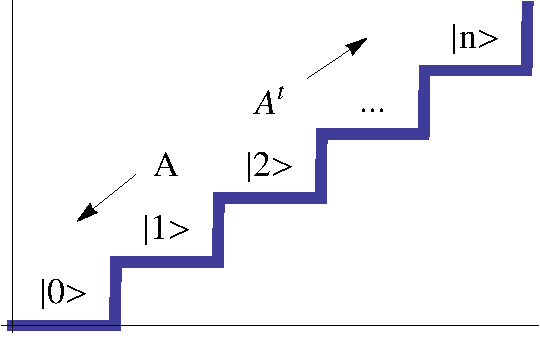
\includegraphics[scale=0.7]{escada}
   \end{center}
 }

\frame{\frametitle{Autoestados}

$$(A^\dagger)^n|0\rangle =C|n\rangle$$

$C$ =?

$$C=\sqrt{n!}$$

$$|n\rangle=\frac{(A^\dagger)^n}{\sqrt{n!}}|0\rangle$$
}

\frame{\frametitle{Funções de onda}

Devemos determinar $\langle n|x\rangle$, as autofunções do operador
Hamiltoniano. 

$$|n\rangle=\frac{(A^{\dagger})^n}{\sqrt{n!}}|0\rangle$$

$$u_n(x)=\frac{1}{\sqrt{n!}}\left\langle x\left| \left(\sqrt{\frac{m\omega}{2\hbar}}\hat{x}+i \sqrt{\frac{1}{2m\omega\hbar}}\hat{p}\right)^n\right|0\right\rangle$$

Para conseguir fazer esse cáculo precisamos de dois ingredientes
$$\langle x|\hat{x}| 0\rangle \quad \langle x|\hat{p}| 0\rangle $$

}


\frame{\frametitle{$\langle x|\hat{x}| 0\rangle$}
$$\langle x|\hat{x}| 0\rangle=x\langle x| 0\rangle=xu_o(x)$$
}

\frame{\frametitle{$\langle x|\hat{p}| 0\rangle$}

$$\langle x|\hat{p}| 0\rangle=
\int dp \langle x| \hat{p} |p\rangle\langle p|0 \rangle$$

$$=\int dp p\langle x |p\rangle\langle p|0 \rangle$$

Interpretando:

$$\int dp pe^{ixp/\hbar} \phi_o(p)=\frac{\hbar}{i}\frac{\partial}{\partial x}
\int dp e^{ixp/\hbar} \phi_o(p)$$

onde $\phi_o (p)$ é a autofunção de energia na representação $p$. 

$$=\frac{\hbar}{i}\frac{\partial}{\partial x}u_o(x)$$
}

 \frame{\frametitle{Funções de onda}

 Devemos determinar $\langle n|x\rangle$, as autofunções do operador
 Hamiltoniano. 

 $$\langle x |n\rangle=\left\langle x \left| \frac{(A^{\dagger})^n}{\sqrt{n!}}\right|0\right\rangle$$

 $$\langle x |n\rangle=\frac{1}{\sqrt{n!}}\left\langle x \left|  \left(\sqrt{\frac{m\omega}{2\hbar}}\hat{x}-i \sqrt{\frac{1}{2m\omega\hbar}}\hat{p}\right)^n\right|0\right\rangle$$
 Com alguma dose de fé:


 $$\frac{1}{\sqrt{n!}}\left(\sqrt{\frac{m\omega}{2\hbar}}x-\sqrt{\frac{\hbar}{2m\omega}}\frac{\partial}{\partial x}\right) ^nu_o(x)$$
 }

 \frame{\frametitle{Funções de onda: $u_o(x)$}


$$Au_o(x)=0$$

$$ \left(\sqrt{\frac{m\omega}{2\hbar}}x+\sqrt{\frac{\hbar}{2m\omega}}\frac{\partial}{\partial x}\right)u_o(x)=0$$

Resolvendo esta equação temos que:

$$u_o=\left( \frac{m\omega}{\pi\hbar} \right)^{(1/4)}e^{-\frac{m\omega x^2}{2\hbar}}$$

Finalmente temos:
 $$u_n=\frac{1}{\sqrt{n!}}\left( \frac{m\omega}{\pi\hbar} \right)^{(1/4)}\left(\sqrt{\frac{m\omega}{2\hbar}}x-\sqrt{\frac{\hbar}{2m\omega}}\frac{\partial}{\partial x}\right) ^n e^{-\frac{m\omega x^2}{2\hbar}}$$


}



 \frame{\frametitle{Dependência temporal dos operadores}
Equação de Schrödinger

$$i\hbar\frac{d}{dt}|\psi(t)\rangle=\hat{H} |\psi(t)\rangle
$$

$$|\psi(t)\rangle=e^{-i\hat{H}t/\hbar}|\psi(0)\rangle$$

$$\langle B\rangle_t=\langle \psi(t)|\hat{B}| \psi(t)\rangle = 
\langle \psi(0)|e^{i\hat{H}t/\hbar}\hat{B}e^{-i\hat{H}t/\hbar}| \psi(t)\rangle
$$

$$\hat{B}(t)=e^{i\hat{H}t/\hbar}\hat{B}e^{-i\hat{H}t/\hbar}$$

``Picture de Heisenberg''
}

 \frame{\frametitle{Picture de Heisenberg}

$$\frac{d\hat{B}(t)}{dt}=\frac{i}{\hbar}e^{i\hat{H}t/\hbar}\hat{H} \hat{B}e^{-i\hat{H}t/\hbar}-\frac{i}{\hbar}e^{i\hat{H}t/\hbar}\hat{B}\hat{H}e^{-i\hat{H}t/\hbar}$$

$$\frac{d\hat{B}(t)}{dt}=\frac{i}{\hbar}[\hat{H},\hat{B}(t)]$$


}

\frame{\frametitle{Exemplo: Oscilador Harmônico}
$$A(t)=e^{i\hat{H}t/\hbar}Ae^{-i\hat{H}t/\hbar}$$
$$A^\dagger(t)=e^{i\hat{H}t/\hbar}A^\dagger e^{-i\hat{H}t/\hbar}$$
$$[A(t),A^\dagger(t)]=1$$
$$[\hat{H},A(t)]=\hbar \omega A(t)$$
$$[\hat{H},A^\dagger(t)]=-\hbar \omega A^\dagger(t)$$
$$\frac{dA(t)}{dt}=-i\omega A(t)$$

$$\frac{dA^\dagger(t)}{dt}=i\omega A^\dagger(t)$$
}

\frame{\frametitle{Exemplo: Oscilador Harmônico}
$$\hat{p}(t)=\hat{p}(0)\cos \omega t -m\omega  \hat{x}(0) \sin \omega t$$
$$\hat{x}(t)=\hat{x}(0)\cos \omega t -\frac{\hat{p}(0)}{m\omega}\hat{x}(0) \sin \omega t$$
}
\end{document}
